%提出するレポートの書式はこのtemplateファイルに沿って作成してください。
%特に表紙・概要の書式は変えないで下さい。

\documentclass[a4j]{jarticle}

\usepackage[dvipdfmx]{graphicx}
% \usepackage{epsbox}
\usepackage{url}
\usepackage{here}
\usepackage{ascmac}

\setlength{\headsep}{-5mm}
\setlength{\oddsidemargin}{0mm}
\setlength{\textwidth}{165mm}
\setlength{\textheight}{230mm}
\setlength{\footskip}{20mm}

\title{
\vspace{30mm}
{\bf 高知工科大学様}\\
\vspace{5mm}
大学掲示板(KUTBBS)\\
\vspace{5mm}
{\bf  内部設計書v1.0}
\vspace{90mm}
}
 \author{
\vspace{5mm}
グループ10 \\
\vspace{5mm}
Pathfinder \\
\vspace{5mm}
\vspace{10mm}
}

 \begin{document}
\maketitle
\newpage
\tableofcontents
\newpage


 \section{システム概要}
本システムは本校の学生同士によって問題提起から問題解決までを匿名で行えるようにするためのシステムである。\\
本システムはWebブラウザ上で「掲示板システム」「ユーザシステム」「管理者システム」によって構築される\\
各要素の主な機能は以下に示す。
\begin{itemize}
\item 掲示板システム
	\begin{itemize}
	\item 掲示板サブシステム
	\item 検索サブシステム
	\item コレクトボタンサブシステム
	\item 通報サブシステム
	\item 通知サブシステム
	\end{itemize}
\item ユーザシステム
	\begin{itemize}
	\item アカウント登録サブシステム
	\item ログインサブシステム
	\item マイページサブシステム
	\item ブックマークサブシステム
	\item お知らせ表示サブシステム
	\end{itemize}
\item 管理者システム
	\begin{itemize}
	\item 管理者ログインサブシステム
	\item 子管理者管理サブシステム
	\item お知らせ編集サブシステム
	\item 掲示板編集サブシステム
	\item ユーザ管理サブシステム
	\end{itemize}
\end{itemize}
 \section{動作環境}
本システムの動作環境は以下の通りである。
\begin{itemize}
\item 動作環境
	\begin{itemize}
	\item CPU : ARM Cortex-A53 1GHz以上
	\item GPU : Broadcom VideoCore IV
	\item メモリ : 2GB以上
	\item ストレージ : 4GB eMMC / SDカードPIN
	\item OS
	\begin{itemize}
		\item Linux version
		\item ubuntu version
		\item MacOS version
		\item Windowss7 , 8 , 10
		\item iOS 10.0
	\end{itemize}
	\item webサーバ : AWS EC2
	\item Appサーバ : Ruby on Rails version 5.1.4
	\item RDBMS : MySQL version 8.0
	\end{itemize}
\item 使用ブラウザ : GoogleChrome62.0 , Firefox version 57.0% , Safari11.0.1
\end{itemize}
\section{開発環境}
本システムの開発環境は以下の通りである。
\begin{itemize}
\item OS : Linux , ubuntu , MacOS , Windows , iOS10.0
\item HTML : version5
\item 使用言語
	\begin{itemize}
	\item ruby version 2.4.2
	\item Ruby on Rails version 5.1.4
	\item CSS
	\item JavaScript
	\end{itemize}
\item サーバ :
\item データベース : MySQL version 8.0
\item webサーバ : AmazonWebServices
\end{itemize}
 \section{内部設計書作成方針}
\subsection{コーディング規約}
\subsubsection{命名規約}
\begin{itemize}
\item 変数名・メソッド名\\
‐ 小文字始まりとする\\
‐ 基本的に意味のある単語を使用する\\
‐
\end{itemize}
\begin{itemize}
\item 定数\\
‐ 全て大文字を使用する\\
\end{itemize}
\begin{itemize}
\item クラス名・構造体名\\
‐ 変数名・メソッド名を同様に意味のある単語を使用する\\
‐ 大文字始まりとする\\
‐ 複数の単語を組み合わせる際は先頭文字を大文字で表記する\\
\end{itemize}
\subsubsection{コーディングスタイル}
\begin{itemize}
\item インデント\\
‐ インデントにはタブを使用する(半角スペース4文字)
\end{itemize}
\begin{itemize}
\item 括弧\\
‐ 中括弧は改行して始める\\
‐ 小括弧の前後にはスペースを使用しない
\end{itemize}
\begin{itemize}
\item 演算子\\
‐ 演算子の前後には半角スペースを一文字使用する
\end{itemize}
\subsection{設計書作成環境}
内部設計書の作成環境は,表\ref{tab:creating_environment}に示します。
\begin{table}[htb]
\caption{内部設計書の作成環境環境}
\begin{center}
  \begin{tabular}{|c|c|} \hline
    組版処理システム & LATEX,dvpdfmx\\ \hline
   文字コード &  UTF-8\\ \hline
    改行コード & LF(0x0A)  \\ \hline
  \end{tabular}
\label{tab:creating_environment}
\end{center}
\end{table}
\subsection{サーバ環境}
本システムを利用するためにはAmazon Web Services(AWS) の EC2 インスタンスを用いて実現します.サーバ環境は表\ref{tab:server_environment}に示します。
\begin{table}[htb]
\caption{サーバ側の動作環境}
\begin{center}
  \begin{tabular}{|c|c|} \hline
    対応OS & Ruby on Rails \\ \hline
   vCPU & 1\\ \hline
    メモリ(GiB) & 1  \\ \hline
    ストレージ & 30GB \\ \hline
  \end{tabular}
\label{tab:server_environment}
\end{center}
\end{table}
\section{データベース設計}
本章では本システムにおけるデータベースMySQLについてを示す。

\subsection{データテーブル構成}
本小節ではデータテーブルの構成をER図を用いて示す。


\begin{figure}[H]
\begin{center}
\resizebox{10cm}{!}{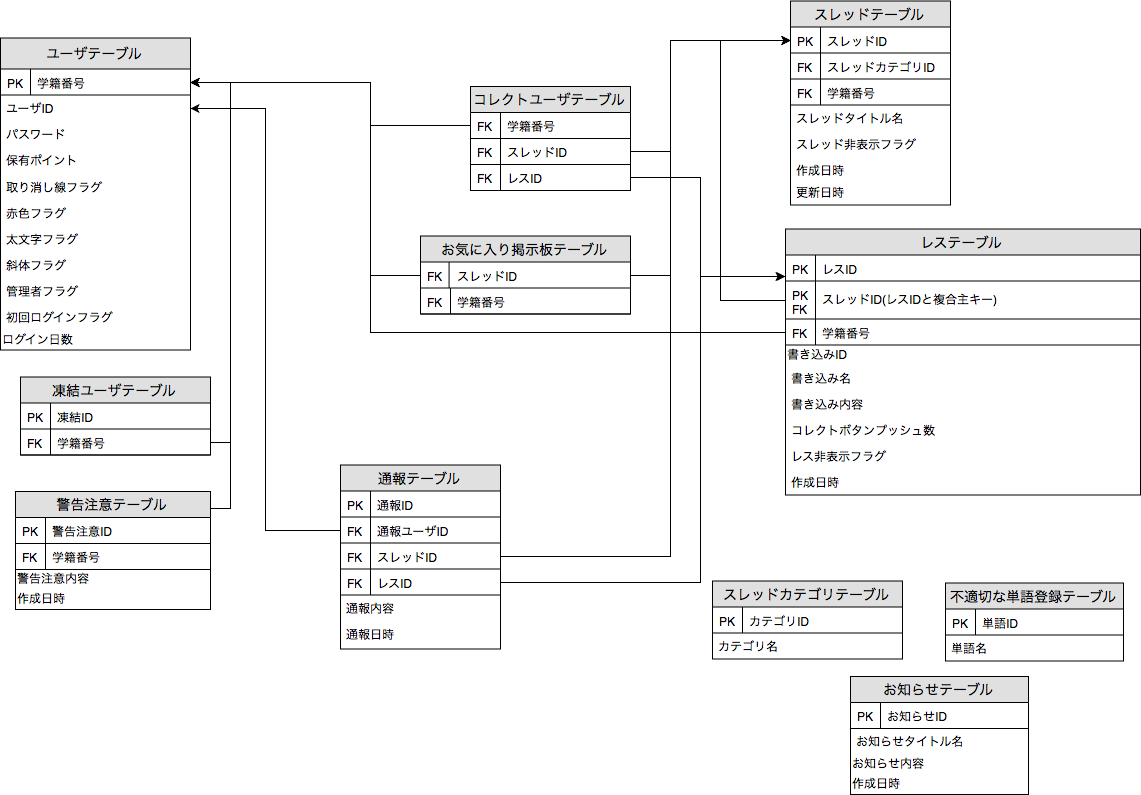
\includegraphics{date-ER1.png}}
\caption{ER図}
\label{}
\end{center}
\end{figure}
\newpage

\subsection{テーブル設計}
本小節ではデータベース構成するテーブルについて示す。また、各カラムについても詳細も示す。

\subsubsection{ユーザテーブル(user)}
ユーザテーブルではユーザに関する情報を管理する。このテーブルの詳細は表\ref{tab:user} に示す。
\begin{table}[h]

  \caption{ユーザテーブル}
  \begin{center}
    \footnotesize
    \begin{tabular}{|l|l|l|c|c|l|l|} \hline

      \multicolumn{1}{|c|}{論理名}&\multicolumn{1}{|c|}{物理名}&\multicolumn{1}{|c|}{データ型}&精度&NULL&\multicolumn{1}{|c|}{オプション}&\multicolumn{1}{|c|}{PK/FK:mode}\\\hline \hline
      学籍番号&student\verb|_|id&char&7&×&-&\multicolumn{1}{|l|}{PK} \\\hline
      ユーザID&user\verb|_|id&varchar&20&×&-&- \\ \hline
      パスワード&password&varchar&20&×&-&- \\ \hline
      保有ポイント&now\verb|_|point&int&4&×&-&- \\ \hline
      取り消しフラグ&cancel\verb|_|flag&int&1&×&-&- \\ \hline
      赤色フラグ&color\verb|_|flag&int&1&×&-&- \\ \hline
      斜体フラグ&diagonal\verb|_|flag&int&1&×&-&- \\ \hline
      太文字フラグ&bold\verb|_|letters\verb|_|flag&int&1&×&-&- \\ \hline
      管理者フラグ&administrator\verb|_|flag&int&1&○&-&- \\ \hline
      初回ログインフラグ&first\verb|_|login\verb|_|flag&int&1&×&-&- \\ \hline
      ログイン日数&count\verb|_|login&int&4&×&-&-\\ \hline 
    \end{tabular}
    \label{tab:user}
  \end{center}
\end{table}

\begin{itemize}
\item 学籍番号\\
  ユーザの学籍番号を示す値であり、自テーブルの主キーである。NULL値は含まない。値は固定7文字の半角英数字にて構成される。\\
\item ユーザID\\
  ユーザを識別するためのIDを示す値である。NULL値は含まない。値は20文字以下の半角英数字にて構成される。
\item パスワード\\
  ユーザを識別するためのパスワードを示す値である。NULL値は含まない。値は20文字以下の半角英数字にて構成される。\\
\item 保有ポイント\\
  ユーザがログインした日数とコレクトボタンを10回以上押されたことで獲得したポイントを示す値である。NULL値は含まない。4桁(0001から9999)の数値にて構成される。

\item 取り消しフラグ\\
  拡張機能の1つであり、取り消し線を付与することを示す値である。NULL値は含まない。値は1桁の0(OFF)、1(ON)の数値にて構成される。\\
  
\item 赤色フラグ\\
  拡張機能の1つであり、赤色を付与することを示す値である。NULL値は含まない。値は1桁の0(OFF)、1(ON)の数値にて構成される。\\
\item 斜体フラグ\\
  拡張機能の1つであり、斜体を付与することを示す値である。NULL値は含まない。値は1桁の0(OFF)、1(ON)の数値にて構成される。\\

\item 太文字フラグ\\
  拡張機能の1つであり、太文字を付与することを示す値である。NULL値は含まない。値は1桁の0(OFF)、1(ON)の数値にて構成される。\\

\item 管理者フラグ\\
  親管理者と子管理者を識別することを示す値である。値は1桁の0(子管理者)、1(親管理者)の数値にて構成される。\\
\item 初回ログインフラグ\\
  初回ログインを識別することを示す値である。NULL値は含まない。値は1桁の0(OFF)、1(ON)の数値にて構成される。
  
\item ログイン日数\\
  ユーザがログインをした日数を記録することを示す値である。NULL値は含まない。値は4桁(0001から9999)の数値にて構築される。
  
   \end{itemize}
\newpage
  \subsubsection{スレッドテーブル(thread)}
  スレッドテーブルではスレッドに関する情報を管理する。このテーブルの詳細は表\ref{tab:thread} に示す。
  \begin{table}[h]
    \caption{スレッドテーブル}
    \begin{center}
      %\fontsize{6.5pt}{30pt}\selectfont
      \footnotesize
      \begin{tabular}{|l|l|l|c|c|l|l|} \hline
        \multicolumn{1}{|c|}{論理名}&\multicolumn{1}{|c|}{物理名}&\multicolumn{1}{|c|}{データ型}&精度&NULL&\multicolumn{1}{|c|}{オプション}&\multicolumn{1}{|c|}{PK/FK:mode}\\\hline \hline
        スレッドID&thread\verb|_|id&int&5&×&\begin{tabular}{l}unsigned zerofill\\auto\verb|_|increment\end{tabular}&\multicolumn{1}{|l|}{PK} \\\hline
          スレッドカテゴリID&thread\verb|_|category\verb|_|id&int&3&×&\begin{tabular}{l}unsigned zerofill\\auto\verb|_|increment\end{tabular}&FK:thread\verb|_|category \\ \hline
            学籍番号&student\verb|_|id&char&7&×&-&\multicolumn{1}{|l|}{FK:user} \\\hline
            スレッドタイトル名&thread\verb|_|category\verb|_|name&varchar&50&×&-&- \\ \hline
            スレッド非表示フラグ&thread\verb|_|hide\verb|_|flag&int&1&×&-&- \\ \hline
            作成日時&created\verb|_|at&timestamp&-&×&default current\verb|_|timestamp&- \\ \hline
            更新日時&updated\verb|_|at&timestamp&-&×&\begin{tabular}{l}default current\verb|_|timestamp on \\update current\verb|_|timestamp\end{tabular}&- \\ \hline
      \end{tabular}
      
      \label{tab:thread}
    \end{center}
  \end{table}
  \begin{itemize}  
  \item スレッドID\\
    自テーブルの主キーである。NULL値は含まない。値は5桁(00001から99999)の数値にて構成され自動追加される。\\

  \item スレッドカテゴリID\\
    スレッドカテゴリテーブルを参照する際の外部キーである。NULL値は含まない。値は3桁(001から999)の数値にて構成され自動追加される。\\
    
  \item 学籍番号\\
    ユーザテーブルを参照する際の外部キーである。NULL値は含まない。固定7文字の半角英数字にて構成される。\\
    
  \item スレッドタイトル名\\
    スレッドタイトルを示す値である。NULL値は含まない。値は50文字以下の文字列にて構成される。\\
  \item スレッド非表示フラグ\\
    管理者の操作権限でスレッドを非表示を示す値である。NULL値は含まない。値は1桁の数値で0(OFF)、1(ON)の数値にて構成される。\\
    例としてスレッド非表示フラグを1にした場合、ユーザ側からはスレッドが非表示になる。
  \item 作成日時\\
    レコードを作成した日付・時刻を示す値である。NULL値は含まない。レコードが作成されるたびに自動追加を行う。
  \item 更新日時\\
    レコードを更新した日付・時刻を示す値である。NULL値は含まない。レコードが更新されるたびに自動更新を行う。
  \end{itemize}
  \subsubsection{レステーブル(res)}
  レステーブルではレスに関する情報を管理する。このテーブルの詳細は表\ref{tab:ress} に示す。
  \begin{table}[h]
    \caption{レステーブル}
    \begin{center}
      %\fontsize{6.5pt}{30pt}\selectfont
      \footnotesize
      \begin{tabular}{|l|l|l|c|c|l|l|} \hline
        \multicolumn{1}{|c|}{論理名}&\multicolumn{1}{|c|}{物理名}&\multicolumn{1}{|c|}{データ型}&精度&NULL&\multicolumn{1}{|c|}{オプション}&\multicolumn{1}{|c|}{PK/FK:mode}\\\hline \hline
        レスID&res\verb|_|id&int&4&×&\begin{tabular}{l}unsigned zerofill\\auto\verb|_|increment\end{tabular}&PK \\\hline
          スレッドID&thread\verb|_|id&int&5&×&\begin{tabular}{l}unsigned zerofill\\auto\verb|_|increment\end{tabular}&\begin{tabular}{l}PK(res複合)\\FK:thread\end{tabular}\\\hline
              学籍番号&student\verb|_|id&char&7&×&-&\multicolumn{1}{|l|}{FK:user} \\\hline
              書き込みID&write\verb|_|id&char&8&×&-&-\\ \hline 
              書き込み名&write\verb|_|name&varchar&15&×&-&- \\ \hline
              書き込み内容&write\verb|_|content&varchar&200&×&-&- \\ \hline
              コレクトプッシュ数&collect\verb|_|push\verb|_|count&int&4&×&-&- \\ \hline
              書き込みID&write\verb|_|id&char&8&×&-&-\\ \hline 
              レス非表示フラグ&res\verb|_|hide\verb|_|flag&int&1&×&-&- \\ \hline
              作成日時&created\verb|_|at&timestamp&-&×&default current\verb|_|timestamp&- \\ \hline
      \end{tabular}
      
      \label{tab:ress}
    \end{center}
  \end{table}
  
  \begin{itemize}
  \item レスID\\
    自テーブルの主キーである。NULL値は含まない。値は4桁(0001から9999)の数値にて構成され自動追加される。
  \item スレッドID\\
    スレッドテーブルを参照する際の外部キーであり、スレIDとの複合主キーである。NULL値は含まない。値は5桁(00001から99999)の数値にて構成され自動追加される。
  \item 学籍番号\\
    ユーザテーブルを参照する際の外部キーである。NULL値は含まない。固定7文字の半角英数字にて構成される。\\
  \item 書き込みID\\
    ユーザが書き込みを行う際に表示するIDを示す値である。NULL値は含まない。値は固定8文字の半角英数字にて構成される。\\   
  \item 書き込み名\\
    書き込みを行う際に表示する名前を示す値である。NULL値は含まない。値は15文字以下の文字列にて構成される。\\
  \item 書き込み内容\\
    書き込み内容を示す値である。NULL値は含まない。値は200文字以下の文字列にて構成される。\\
  \item コレクトボタンプッシュ数\\
    レスに対してコレクトボタンが押された回数を示す値である。NULL値は含まない。値は4桁(0001から9999)の数値にて構成される。\\
  \item レス非表示フラグ\\
    管理者の操作権限でレスを非表示を示す値である。NULL値は含まない。値は1桁の数値で0(OFF)、1(ON)の数値にて構成される。\\
    例としてレス非表示フラグを1にした場合、ユーザ側からはレスが非表示になる。
    
  \item 作成日時\\
    レコードを作成した日付・時刻を示す値である。NULL値は含まない。レコードが作成されるたびに自動追加される。    
  \end{itemize}

  \subsubsection{スレッドカテゴリテーブル(thread\_category)}
  スレッドカテゴリテーブルは各カテゴリごとに分けられたスレッドの情報を管理する。このテーブルの詳細は表\ref{tab:thread_category} に示す。
  \begin{table}[h]
    \caption{スレッドカテゴリテーブル}
    \begin{center}
      %\fontsize{6.5pt}{30pt}\selectfont
      \footnotesize
      \begin{tabular}{|l|l|l|c|c|l|l|} \hline
        \multicolumn{1}{|c|}{論理名}&\multicolumn{1}{|c|}{物理名}&\multicolumn{1}{|c|}{データ型}&精度&NULL&\multicolumn{1}{|c|}{オプション}&\multicolumn{1}{|c|}{PK/FK:mode}\\\hline \hline
        カテゴリID&category\verb|_|no&int&3&×&\begin{tabular}{l}unsigned zerofill\\auto\verb|_|increment\end{tabular}&PK\\ \hline
          カテゴリ名&category\verb|_|name&varchar&15&×&-&-\\\hline
      \end{tabular}
      \label{tab:thread_category}
    \end{center}
  \end{table}
  
  \begin{itemize}
  \item カテゴリID\\
    自テーブルの主キーである。NULL値は含まない。値は3桁(001から999)の数値にて構築され自動追加される。
  \item カテゴリ名\\
    カテゴリの名前を示す値である。NULL値は含まない。値は15文字以下の文字列にて構成される。\\
    
  \end{itemize}

  \subsubsection{お気に入り掲示板テーブル(favorite\_bbs)}
  お気入り掲示板テーブルではブックマークとして登録したスレッド情報を管理する。このテーブルの詳細は表\ref{tab:favorite_bbs} に示す。
  \begin{table}[h]
    \caption{お気に入り掲示板テーブル}
    \begin{center}
      %\fontsize{6.5pt}{30pt}\selectfont
      \footnotesize
      \begin{tabular}{|l|l|l|c|c|l|l|} \hline
        \multicolumn{1}{|c|}{論理名}&\multicolumn{1}{|c|}{物理名}&\multicolumn{1}{|c|}{データ型}&精度&NULL&\multicolumn{1}{|c|}{オプション}&\multicolumn{1}{|c|}{PK/FK:mode}\\\hline \hline
        学籍番号&student\verb|_|id&char&7&×&-&\multicolumn{1}{|l|}{FK:user} \\\hline
        スレッドID&thread\verb|_|id&int&5&×&\begin{tabular}{l}unsigned zerofill\\auto\verb|_|increment\end{tabular}&FK:thread\\\hline
      \end{tabular}
      \label{tab:favorite_bbs}
    \end{center}
  \end{table}
  
  \begin{itemize}
  \item 学籍番号\\
    ユーザテーブルを参照する際の外部キーである。NULL値は含まない。固定7文字の半角英数字にて構成される。\\
  \item スレッドID\\
    スレッドテーブルを参照する際の外部キーである。NULL値は含まない。値は5桁(00001から99999)の数値にて構築され自動追加される。
  \end{itemize}
  
  
  
  \subsubsection{コレクトユーザテーブル(collect\_user)}
  コレクトユーザテーブルではコレクトボタンを押されたことに関する情報を管理する。このテーブルの詳細は表 \ref{tab:collect_user} に示す。
  \begin{table}[h]
    \caption{コレクトユーザテーブル}
    \begin{center}
      %\fontsize{6.5pt}{30pt}\selectfont
      \footnotesize
      \begin{tabular}{|l|l|l|c|c|l|l|} \hline
        \multicolumn{1}{|c|}{論理名}&\multicolumn{1}{|c|}{物理名}&\multicolumn{1}{|c|}{データ型}&精度&NULL&\multicolumn{1}{|c|}{オプション}&\multicolumn{1}{|c|}{PK/FK:mode}\\\hline \hline
        学籍番号&student\verb|_|id&char&7&×&-&\multicolumn{1}{|l|}{FK:user} \\\hline
        スレッドID&thread\verb|_|id&int&5&×&\begin{tabular}{l}unsigned zerofill\\auto\verb|_|increment\end{tabular}&FK:thread\\\hline
          レスID&res\verb|_|no&int&4&×&\begin{tabular}{l}unsigned zerofill\\auto\verb|_|increment\end{tabular}&FK:res \\\hline
      \end{tabular}
      \label{tab:collect_user}
    \end{center}
  \end{table}

  \begin{itemize}
  \item 学籍番号\\
    ユーザテーブルを参照する際の外部キーである。NULL値は含まない。固定7文字の半角英数字にて構成される。\\
  \item スレッドID\\
    スレッドテーブルを参照する際の外部キーである。NULL値は含まない。値は5桁(00001から99999)の数値にて構成され自動追加される。
  \item レスID\\
    レステーブルを参照する際の外部キーである。NULL値は含まない。値は4桁(0001から9999)の数値にて構成され自動追加される。
  \end{itemize}

  \subsubsection{不適切な単語登録テーブル(inadequacy\_word)}
  不適切な単語登録テーブルでは管理者が誹謗中傷や公序良俗に違反していると考えられる単語を登録した情報を管理する。このテーブルの詳細は表 \ref{tab:inadequacy_word} に示す。
  \begin{table}[h]
    \caption{不適切な単語登録テーブル}
    \begin{center}
      %\fontsize{6.5pt}{30pt}\selectfont
      \footnotesize
      \begin{tabular}{|l|l|l|c|c|l|l|} \hline
        \multicolumn{1}{|c|}{論理名}&\multicolumn{1}{|c|}{物理名}&\multicolumn{1}{|c|}{データ型}&精度&NULL&\multicolumn{1}{|c|}{オプション}&\multicolumn{1}{|c|}{PK/FK:mode}\\\hline \hline
        単語ID&word\verb|_|id&int&5&×&\begin{tabular}{l}unsigned zerofill\\auto\verb|_|increment\end{tabular}&PK\\\hline
          単語名&word\verb|_|name&varchar&200&×&-&- \\\hline
      \end{tabular}
      \label{tab:inadequacy_word}
    \end{center}
  \end{table}
  
  \begin{itemize}
  \item 単語ID\\
    自テーブルの主キーである。NULL値は含まない。値は5桁(00001から99999)の数値にて構成され自動追加される。
  \item 単語名\\
    管理者の操作権限で登録した単語を示す値である。NULL値は含まない。値は200文字以下の文字列にて構成される。
  \end{itemize}

  
  \subsubsection{通報テーブル(report)}
  通報テーブルではユーザが誹謗中傷や公序良俗に違反するなどの不適切な内容であると判断したスレッドまたはレスを管理者に通報した時の情報を管理する。また、通報した内容の情報も管理する。このテーブルの詳細は表 \ref{tab:report} に示す。
  \begin{table}[h]
    \caption{通報テーブル}
    \begin{center}
      %\fontsize{6.5pt}{30pt}\selectfont
      \footnotesize
      \begin{tabular}{|l|l|l|c|c|l|l|} \hline
        \multicolumn{1}{|c|}{論理名}&\multicolumn{1}{|c|}{物理名}&\multicolumn{1}{|c|}{データ型}&精度&NULL&\multicolumn{1}{|c|}{オプション}&\multicolumn{1}{|c|}{PK/FK:mode}\\\hline \hline
        通報ID&report\verb|_|id&int&5&×&\begin{tabular}{l}unsigned zerofill\\auto\verb|_|increment\end{tabular}&PK\\\hline
          通報ユーザID&report\verb|_|user\verb|_|id&varchar&20&×&-&FK:user \\ \hline
          スレッドID&thread\verb|_|id&int&5&×&\begin{tabular}{l}unsigned zerofill\\auto\verb|_|increment\end{tabular}&FK:thread\\\hline
            レスID&res\verb|_|id&int&4&×&\begin{tabular}{l}unsigned zerofill\\auto\verb|_|increment\end{tabular}&FK:res \\\hline
              通報内容&report\verb|_|content&varchar&200&×&-&-\\ \hline
              通報日時&report\verb|_|at&timestamp&-&×&default current\verb|_|timestamp&- \\ \hline
      \end{tabular}
      \label{tab:report}
    \end{center}
  \end{table}
  
  \begin{itemize}
  \item 通報ID\\
    自テーブルの主キーである。NULL値は含まない。値は5桁(00001から99999)の数値にて構成され自動追加される。
  \item 通報ユーザID\\
    ユーザテーブルを参照する際の外部キーである。NULL値は含まない。値は20文字以下の半角英数字にて構成される。\\

  \item スレッドID\\
    スレッドテーブルを参照する際の外部キーである。NULL値は含まない。値は5桁(00001から99999)の数値にて構成され自動追加される。
  \item レスID\\
    レステーブルを参照する際の外部キーである。NULL値は含まない。値は4桁(0001から9999)の数値にて構成され自動追加される。
  \item 通報内容\\
    通報内容を示す値である。NULL値は含まない。値は200文字以下の文字列にて構成される。\\
    
  \item 通報日時\\
    レコードを作成した日付・時刻を示す値である。NULL値は含まない。レコードが作成されるたびに自動追加を行う。
  \end{itemize}
  
  \subsubsection{凍結ユーザテーブル(suspend)}
  凍結ユーザテーブルでは迷惑行為が改善されないユーザのアカウントを凍結した情報を管理する。このテーブルの詳細は表 \ref{tab:suspend} に示す。
  
  \begin{table}[h]
    \caption{凍結ユーザテーブル}
    \begin{center}
      \fontsize{6.5pt}{30pt}\selectfont
      \footnotesize
      \begin{tabular}{|l|l|l|c|c|l|l|} \hline
        \multicolumn{1}{|c|}{論理名}&\multicolumn{1}{|c|}{物理名}&\multicolumn{1}{|c|}{データ型}&精度&NULL&\multicolumn{1}{|c|}{オプション}&\multicolumn{1}{|c|}{PK/FK:mode}\\\hline \hline
        凍結ID&suspend\verb|_|id&int&4&×&\begin{tabular}{l}unsigned zerofill\\auto\verb|_|increment\end{tabular}&PK\\\hline
          学籍番号&student\verb|_|id&char&7&×&-&\multicolumn{1}{|l|}{FK:user} \\\hline
      \end{tabular}
      \label{tab:suspend}
    \end{center}
  \end{table}
  
  \begin{itemize}
  \item 凍結ID\\
    自テーブルの主キーである。NULL値は含まない。値は4桁(0001から9999)の数値にて構成され自動追加される。
  \item 学籍番号\\
    ユーザテーブルを参照する際の外部キーである。。NULL値は含まない。値は固定7文字の半角英数字にて構成される。\\
  \end{itemize}
  
  \subsubsection{お知らせテーブル(news)}
  お知らせテーブルではお知らせに関する情報を管理する。このテーブルの詳細は表 \ref{tab:news} に示す。
  \begin{table}[h]
    \caption{お知らせテーブル}
    \begin{center}
      \fontsize{6.5pt}{30pt}\selectfont
      \footnotesize
      \begin{tabular}{|l|l|l|c|c|l|l|} \hline
        \multicolumn{1}{|c|}{論理名}&\multicolumn{1}{|c|}{物理名}&\multicolumn{1}{|c|}{データ型}&精度&NULL&\multicolumn{1}{|c|}{オプション}&\multicolumn{1}{|c|}{PK/FK:mode}\\\hline \hline
        お知らせID&news\verb|_|id&int&5&×&\begin{tabular}{l}unsigned zerofill\\auto\verb|_|increment\end{tabular}&PK\\\hline
          お知らせタイトル名&news\verb|_|title&varchar&50&×&-&-\\\hline
          お知らせ内容&news\verb|_|title&varchar&400&×&-&-\\\hline
          作成日時&created\verb|_|at&timestamp&-&×&default current\verb|_|timestamp&- \\ \hline
          
      \end{tabular}
      \label{tab:news}
    \end{center}
  \end{table}
  
  \begin{itemize}
  \item お知らせID\\
    自テーブルの主キーである。NULL値は含まない。値は5桁(00001から99999)の数値にて構成され自動追加される。
  \item お知らせタイトル名\\
    お知らせタイトルを示す値である。NULL値は含まない。値は50文字以下の文字列にて構成される。
  \item お知らせ内容\\
    お知らせ内容を示す値である。NULL値は含まない。値は400文字以下の文字列にて構成される。\\

  \item 作成日時\\
    レコードを作成した日付・時刻を示す値である。NULL値は含まない。レコードが作成されるたびに自動追加を行う。    
  \end{itemize}
  \subsubsection{警告注意テーブル(warned\_caution)}
  警告テーブルでは管理者がユーザに対しての警告・注意喚起に関する情報を管理する。このテーブルの詳細は表 \ref{tab:warned_caution} に示す。
  \begin{table}[h]
    \caption{警告注意テーブル}
    \begin{center}
      \fontsize{6.5pt}{30pt}\selectfont
      \footnotesize
      \begin{tabular}{|l|l|l|c|c|l|l|} \hline
        \multicolumn{1}{|c|}{論理名}&\multicolumn{1}{|c|}{物理名}&\multicolumn{1}{|c|}{データ型}&精度&NULL&\multicolumn{1}{|c|}{オプション}&\multicolumn{1}{|c|}{PK/FK:mode}\\\hline \hline
        警告注意ID&warned\verb|_|caution\verb|_|id&int&4&×&\begin{tabular}{l}unsigned zerofill\\auto\verb|_|increment\end{tabular}&PK\\\hline
          学籍番号&student\verb|_|id&char&7&×&-&\multicolumn{1}{|l|}{FK:user} \\\hline

          警告注意タイトル名&warned\verb|_|caution\verb|_|title&varchar&50&×&-&-\\\hline
          警告注意内容&warned\verb|_|caution\verb|_|title&varchar&400&×&-&-\\\hline
          作成日時&created\verb|_|at&timestamp&-&×&default current\verb|_|timestamp&- \\ \hline
          
      \end{tabular}
      \label{tab:warned_caution}
    \end{center}
  \end{table}

  \begin{itemize}
  \item 警告注意ID\\
    自テーブルの主キーである。NULL値は含まない。値は4桁(0001から9999)の数値にて構成され自動追加される。
  \item 学籍番号\\
    ユーザテーブルを参照する際の外部キーである。NULL値は含まない。値は固定7文字の半角英数字にて構成される。\\
    
  \item 警告注意タイトル名\\
    警告注意タイトルを示す値である。NULL値は含まない。値は50文字以下の文字列にて構成される。
  \item 警告注意内容\\
    警告注意内容を示す値である。NULL値は含まない。値は400文字以下の文字列にて構成される。\\
    
  \item 作成日時\\
    レコードを作成した日付・時刻を示す値である。NULL値は含まない。レコードが作成されるたびに自動追加を行う。
  \end{itemize}



\section{モジュール設計}
\subsection{admin\_top.html}
\noindent
【名称】\\
管理者TOP画面\\
【概要】\\
管理者がログインを済ませると最初に現れる画面である。ここでは管理者に与えられた権限の選択をすることができる。\\
【処理フロー】
\begin{itemize}
\item 「掲示板はこちらボタン」を押すと、が呼び出される。
\item 「子管理者管理ボタン」を押すと、admin\_child\_top.htmlが呼び出される。
\item 「ユーザ管理ボタン」を押すと、が呼び出される。
\item 「お知らせ編集ボタン」を押すと、が呼び出される。
\item 「通報状況確認ボタン」を押すと、が呼び出される。
\item 「不適切な単語登録ボタン」を押すと、が呼び出される。
\end{itemize}

\subsection{admin\_child\_top.html}
\noindent
【名称】\\
子管理者管理TOP\\
【概要】\\
各子管理者について発行・抹消を行うための画面である。\\
【処理フロー】
\begin{itemize}
\item 「子管理者アカウント発行ボタン」を押すと、create\_admin.htmlが呼び出される。
\item 「子管理者抹消ボタン」を押すと、delete\_admin.htmlが呼び出される。
\item 「管理者TOPボタン」を押すと、admin\_top.htmlが呼び出される。
\end{itemize}

\subsection{create\_admin.html}
\noindent
【名称】\\
子管理者アカウント発行画面\\
【概要】\\
子管理者アカウントの発行を行うかどうかを決定する画面である。\\
【処理フロー】
\begin{itemize}
\item 「はいボタン」を押すと、.html.erbで処理が行われる。
\item .html.erbで新たなアカウントの発行が完了するとnew\_admin.htmlが呼び出される。
\item 「いいえボタン」を押すと、admin\_child\_top.htmlが呼び出される。
\end{itemize}

\subsection{new\_admin.html}
\noindent
【名称】\\
子管理者アカウント発行完了画面\\
【概要】\\
子管理者アカウント発行完了画面が表示される\\
【処理フロー】
\begin{itemize}
\item 「確認ボタン」を押すと、admin\_child\_top.htmlが呼び出される。
\item 「管理者TOPボタン」を押すと、admin\_top.htmlが呼び出される。
\end{itemize}

\subsection{delete\_admin.html}
\noindent
【名称】\\
子管理者アカウント抹消画面\\
【概要】\\
特定の子管理者アカウントについて抹消するかどうかを決定する画面である。\\
【処理フロー】
\begin{itemize}
\item 「はいボタン」を押すと、.html.erbで処理が行われる
\item .html.erbで子管理者アカウントの抹消が完了するとdelete\_admin\_ok.htmlが呼び出される。
\item 「いいえボタン」を押すと、admin\_child\_top.htmlが呼び出される。
\end{itemize}

\subsection{delete\_admin\_ok.html}
\noindent
【名称】\\
子管理者アカウント抹消完了画面\\
【概要】\\
子管理者アカウント抹消完了画面が表示される\\
【処理フロー】
\begin{itemize}
\item 「戻るボタン」を押すと、admin\_child\_top.htmlが呼び出される。
\end{itemize}

\subsection{user\_admin\_top.html}
\noindent
【名称】\\
ユーザ管理画面\\
【概要】\\
ユーザのアカウント発行とユーザ情報検索を行うことができる画面である。\\
【処理フロー】
\begin{itemize}
\item 「ユーザアカウント発行ボタン」を押すと、create\_user.htmlが呼び出される。
\item 「ユーザ情報検索ボタン」を押すと、search\_user.htmlが呼び出される。
\end{itemize}

\subsection{create\_user.html}
\noindent
【名称】\\
ユーザアカウント発行画面\\
【概要】\\
ユーザアカウントの発行を行うことができる画面である。学籍番号の開始番号と末尾番号を入力することで範囲を指定し、同時に複数のアカウントの発行を行う。\\
【処理フロー】
\begin{itemize}
\item 「開始番号テキストボックス」に新しく発行するユーザの開始番号を入力する。
\item 「末尾番号テキストボックス」に新しく発行するユーザの末尾番号を入力する。
\item 「登録ボタン」を押すと、.html.erbで処理が行われる。
\item .html.erbでユーザのアカウント発行が完了するとnew\_user.htmlが呼び出される。
\item 「管理者TOPボタン」を押すと、admin\_top.htmlが呼び出される。
\end{itemize}

\subsection{new\_user.html}
\noindent
【名称】\\
ユーザアカウント発行確認画面\\
【概要】\\
ユーザアカウント発行確認画面が表示される\\
【処理フロー】
\begin{itemize}
\item 「確認ボタン」を押すと、user\_admin\_top.htmlが呼び出される。
\end{itemize}

\subsection{search\_user.html}
\noindent
【名称】\\
ユーザ情報検索画面\\
【概要】\\
【処理フロー】
\begin{itemize}
\item 「学籍番号検索テキストボックス」にはユーザの情報を入手する際に学籍番号を入力する。
\item 「検索ボタン」を押すと、.html.erbで処理が行われる。
\item .html.erbで該当するユーザがあればuser\_info.htmlが呼び出される。
\end{itemize}

\subsection{user\_info.html}
\noindent
【名称】\\
ユーザ情報画面\\
【概要】\\
ユーザ情報の検索結果を表示する画面である。
【処理フロー】
\begin{itemize}
\item 「警告・注意喚起ボタン」を押すと、が呼び出される。
\item 「アカウント凍結ボタン」を押すと、が呼び出される。
\item 「パスワード表示ボタン」を押すと、が呼び出される。
\item 「管理者TOPボタン」を押すと、admin\_top.htmlが呼び出される。
\end{itemize}

\subsection{.html}
\noindent
【名称】\\
画面\\
【概要】\\
【処理フロー】
\begin{itemize}
\item 「ボタン」を押すと、が呼び出される。
\end{itemize}

\subsection{login\_top.html}
【名称】\\
ログインTOP画面\\
【概要】\\
利用者が本システムを利用する際の初期画面である。ここでは、ユーザとしてログイン、管理者としてログインのいずれかを選択することができる。\\
【処理フロー】
\begin{itemize}
  \item ログインボタンを押すとlogin\_user.htmlが呼び出される。
  \item 管理者はこちらボタンを押すとlogin\_admin.htmlが呼び出される。
\end{itemize}

%ユーザ側
\subsection{login\_user.html}
【名称】\\
ユーザログイン画面\\
【概要】\\
ユーザがIDとパスワードを入力して本システムにログインするための画面である。\\
【処理フロー】\\
\begin{itemize}
  \item 「ID入力テキストボックス」にユーザのIDを入力する。
  \item 「パスワード入力テキストボックス」にユーザのパスワードを入力する。
  \item 初回のログインでは、IDとパスワードが入力された状態で「ENTERボタン」を押すとsubscribe\_user.htmlが呼び出される。
  \item 2回目以降のログインでは、IDとパスワードが入力された状態で「ENTERボタン」を押すとBBS\_top.htmlが呼び出される。
  \item データベース上に存在しないIDまたはパスワードが入力された状態で「ENTERボタン」を押すと、.html.erbが呼び出される。
  \item いずれかのテキストボックスに何も入力されていない状態で「ENTERボタン」を押すと、.html.erbが呼び出される。
\end{itemize}


\subsection{subscribe\_user.html}
【名称】\\
新規登録画面\\
【概要】\\
初回ログインをしたユーザがIDとパスワードを変更し、本システムに本登録する画面である。\\
【処理フロー】\\
\begin{itemize}
  \item 「ID入力テキストボックス」に変更後のユーザIDを入力する。
  \item 「パスワード入力テキストボックス」に変更後のユーザのパスワードを入力する。
  \item 「パスワード再確認入力テキストボックス」に「パスワード入力テキストボックス」に入力したものと同じパスワードを入力する。
  \item 「ID」「パスワード」「パスワード再確認」のテキストボックスに文字列が入力されており、かつ「パスワード」と「パスワード再確認」のテキストボックスに入力された文字列が一致した場合において、「登録ボタン」を押すとsubscribe\_ok.htmlが呼び出される。
  \item いずれかのテキストボックスに何も入力されていない状態で「登録ボタン」を押すと、.html.erbが呼び出される。
  \item 「登録ボタン」を押したときに「パスワード」と「パスワード再確認」に入力された文字列が合致しなかった場合、.html.erbが呼び出される。
\end{itemize}


\subsection{subscribe\_ok.html}
【名称】\\
新規登録完了画面\\
【概要】\\
新規登録が完了したことを表示する画面である。\\
【処理フロー】\\
\begin{itemize}
  \item 「利用を開始するボタン」を押すと、BBS\_top.htmlが呼び出される。
\end{itemize}


\subsection{read\_news.html}
【名称】\\
お知らせ画面
【概要】\\
管理者からユーザに対するお知らせの詳細を表示する画面である。\\

%管理者側
\subsection{login\_admin.html}
【名称】\\
管理者ログイン画面\\
【概要】\\
管理者がIDとパスワードを入力して本システムにログインするための画面である。\\
【処理フロー】\\
\begin{itemize}
  \item 「管理者ID入力テキストボックス」に管理者のIDを入力する。
  \item 「管理者パスワード入力テキストボックス」に管理者のパスワードを入力する。
  \item 入力されたIDとパスワードがともにデータベースに登録されたものと合致している場合、「ENTERボタン」を押すとadmin\_top.htmlが呼び出される。
  \item 入力されたIDとパスワードのいずれかがデータベースに登録されているものと合致しない場合、「ENTERボタン」を押すと、.html.erbが呼び出される。
  \item IDとパスワードのいずれかが入力されていない場合、「ENTERボタン」を押すと、.html.erbが呼び出される。
\end{itemize}

\subsection{news\_edit.html}
【名称】\\
お知らせ編集画面\\
【概要】\\
管理者がユーザにお知らせを通達する内容を編集する画面である。\\
【処理フロー】\\
\begin{itemize}
  \item お知らせタイトル、内容に文字列が入力されている状態で「送信ボタン」を押すと、news\_edit\_confirm.htmlが呼び出される。
  \item お知らせタイトル、内容のいずれかに文字列が入力されていない状態で「送信ボタン」を押すと、.html.erbが呼び出される。
  \item 「管理者TOPボタン」を押すと、admin\_top.htmlが呼び出される。
\end{itemize}


\subsection{news\_edit\_confirm.html}
【名称】\\
お知らせ内容確認画面\\
【概要】\\
お知らせ編集画面で編集したお知らせ内容を確認する画面である。内容を確認し、送信するか否かを選択する。\\
【処理フロー】\\
\begin{itemize}
  \item 「はいボタン」を押すと、.html.erbが呼び出される。また、news\_edit\_ok.htmlが呼び出される。
  \item 「いいえボタン」を押すと、news\_edit.htmlが呼び出される。
\end{itemize}


\subsection{news\_edit\_ok.html}
【名称】\\
お知らせ作成完了画面\\
【概要】\\
お知らせの作成が完了したことを示す画面である。\\
【処理フロー】\\
\begin{itemize}
  \item 「戻るボタン」を押すとadmin\_top.htmlが呼び出される。
\end{itemize}

%検索画面
\subsection{search.html}
【名称】
\\検索結果画面
\\【概要】
\\利用者が検索を行った際に表示される画面。スレッドタイトルを押すとそのスレッドの閲覧画面が表示される。
\\【処理フロー】
\\\begin{itemize}
\item 「スレッドタイトル」を押すと、read\_thread.htmlを呼び出す。
\end{itemize}

%通報関係
\subsection{report\_reason.html}
【名称】
\\通報画面
\\【概要】
\\利用者が通報ボタンを押した際に表示される画面。
\\【処理フロー】
\\\begin{itemize}
\item 「理由テキストボックス」に通報する理由を入力する。
\item 「送信ボタン」を押すと、report\_confirm.htmlを呼び出す。
\end{itemize}
\subsection{report\_confirm.html}
【名称】
\\通報確認画面
\\【概要】
\\利用者が通報画面にて、「送信ボタン」を押した際に表示される。
\\【処理フロー】
\\\begin{itemize}
\item 「はいボタン」を押すと、report\_ok.htmlを呼び出します。
\item 「いいえボタン」を押すと、report\_reason.htmlを呼び出す。
\\\end{itemize}
\subsection{report\_ok.html}
【名称】
\\通報完了画面
\\【概要】
\\利用者が通報確認画面にて、「はいボタン」を押した際に表示される画面。
\\【処理フロー】
\\\begin{itemize}
  \item 「戻るボタン」を押すとcategory\_top.htmlを呼び出す。
\end{itemize}

%不適切な単語関連
\subsection{NGword.html}
【名称】
\\不適切な単語の登録画面
\\【概要】
\\管理者が掲示板において不適切な単語を登録する画面。「不適切な単語入力テキストボックス」に入力した
単語を「不適切な単語登録ボタン」を押すことで、不適切な単語として登録ができる。
表示されている単語の「削除ボタン」を押すことで、その単語を不適切な単語から外す。
\\【処理フロー】
\\\begin{itemize}
  \item 「不適切な単語入力テキストボックス」に単語を入力し、「不適切な単語登録ボタン」押すことで表示されて
  いる単語の一覧に入力された単語を追加し、(不適切な単語のデータベース)に追加する。
  \item 単語の「削除ボタン」を押すことで、不適切な単語の一覧からその単語を外し、(不適切な単語のデータベース)から外す。
\end{itemize}

\begin{figure}[H]
\begin{center}
\resizebox{8cm}{!}{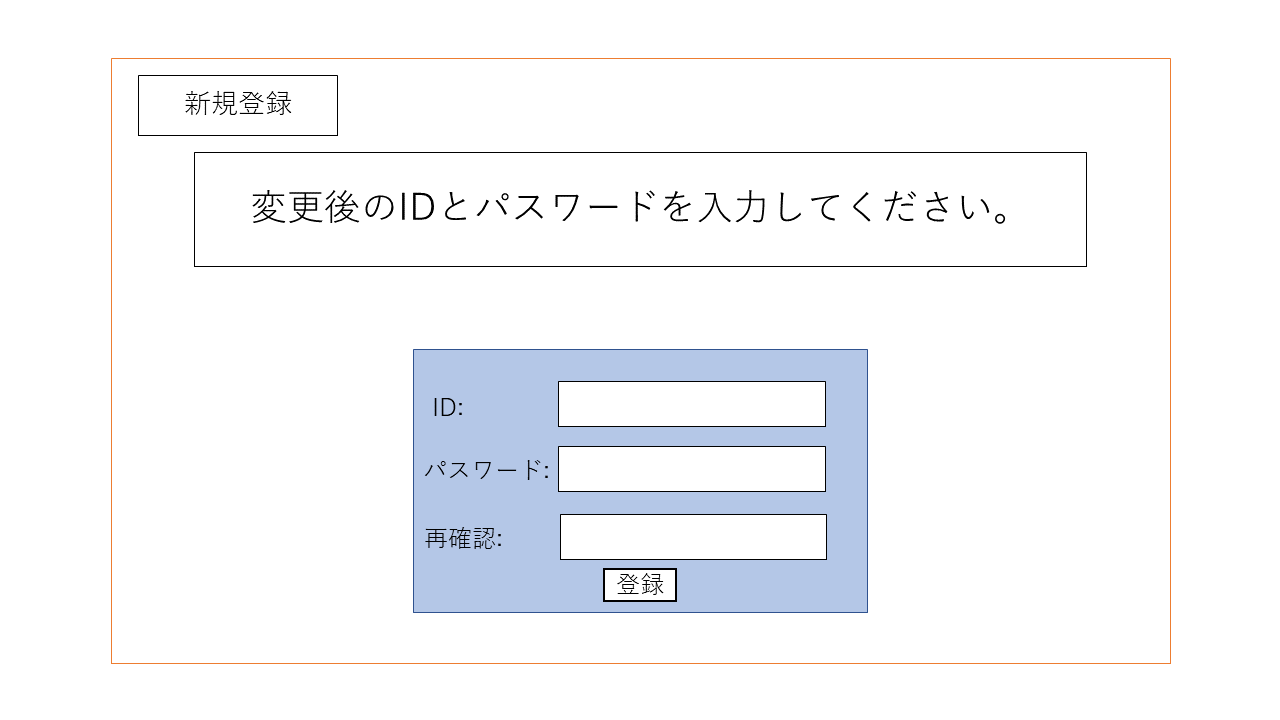
\includegraphics{sequence/subscribe_user.PNG}}
%\caption {カテゴリトップ画面}
%\label {fig:category\_top}
\end{center}
\end{figure}


\section{ルーティング及びMVC一覧}
この章では、Railsの規約に従ったURL規則を示す。また、HTTPメソッドとURLによって呼び出されるControllerとActionを示す。さらに、View及びModelも示す。
\newpage
\subsection{ルーティング一覧}
以下の表は、Railsの規則に従ったURL規則の表である。また、ControllerとそのActionについても示す。



\begin{table}[htb]
  \caption{ルーティング一覧}
  \centering
  \begin{tabular}{|l|l|l||l|} \hline
    No.&   URL 						&METHOD & Controller\#Action \\ \hline \hline
	 1&	/Login  					 	& GET      & sessions\#new       \\
       2&  ~			         			& POST    & sessions\#create	\\
	 3&	/Logout   				      &DELETE   &sessions\#destroy	\\
	 4&	/passwords/:id					&GET	  &passwords\#new    \\
	 5 & /passwords/:id					&PATCH	  &passwords\#change \\
	 6&	/home   						& GET 	   &home\_pages/\#home    \\
       7&	/home   						& PATCH 	   &home\_pages/\#threads\_hide \\
	 8&	/users/:id     					&  GET  	    &  users\#show       \\
	 9&	/users/:id     					 & PATCH   &  users\#update       \\
	10&	/results/:title         			& GET   	    & results\#search      \\
	11& /results/:title/categories/:id		&GET		& categories\#search	\\
	12&	/informations/:id				  & GET       & informations\#show      \\
	13&	/categories/:id    		   		 &   GET      & categories\#index    \\
	14&	/threads/new      	 	  		 &  GET      &  threads\#new         \\
	15&/threads/check      		       &  GET      & threads\#check       \\
	16&/threads                   		       &  POST    &threads\#create      \\
	17&/threads/:id/report\_new   		&   GET      &threads\#report\_new  \\
	18&	/threads/check               		&   GET      & threads\#check       \\
	19&	/threads                      		 & POST     & threads\#create     \\
	20&	/threads/:id/contents      		 &    GET    & contents\#bbs        \\
	21&	/threads/:id/contents/check 	&     GET    &  contents\#check   \\
	22&	/threads/:id/contents          	 &    POST  & contents\#write     \\
	23&	/threads/:id/contents          	 &    PATCH  & contents\#responses\_hide     \\
	24&	/threads/:id/contents/:id/report	 &    GET    & contents\#report    \\
	25&	/threads/:id/contents/:id/check   &   GET    &  contents\#check      \\
	26&	/threads/:id/contents            	 &   POST   & contents\#report\_create \\ \hline

\end{tabular}

\end{table}

\subsection{ルーティング(管理者側)一覧}
※v2でユーザ側と管理者側を統合・修正します。\\
呼び出されたURLとHTTPメソッドによってRailsで呼び出すControllerのアクションを定義する。
\begin{table}[H]
  \centering
  \caption{ルーティング(管理者側)一覧}
  \begin{tabular}{|c|l|l|l|}\hline
    No. & URL & METHOD & Controller\#Action \\ \hline \hline
    1 & admins/login & GET & admins\_session \\
    2 & admins/login & POST & admins\_session\#login \\
    3 & admins/logout & POST & admins\_session\#logout \\ \hline
    4 & admins/top & GET & admins\_top\#home \\ \hline
    5 & admins/ng\_word & GET & ng\_word\#home \\
    6 & admins/ng\_word/create & POST & ng\_word\#create \\
    7 & admins/ng\_word/destroy & DELETE & ng\_word\#destroy \\ \hline
    8 & admins/manage & GET & manage\#home \\
    9 & admins/manage/signup & GET & manage\#signup \\
    10 & admins/manage/create & POST & manage\#create \\
    11 & admins/manage/ok & GET & manage\#ok \\
    12 & admins/manage/destroy\_check & GET & manage\#destroy\_check \\
    13 & admins/manage/destroy & DELETE & manage\#destroy \\ \hline
    14 & admins/manage\_user & GET & manage\_user\#home \\
    15 & admins/manege\_user/signup & GET & manage\_user\#user\_signup \\
    16 & admins/manage\_user/create & POST & manage\_user\#user\_create \\
    17 & admins/manage\_user/search & GET & manage\_user\#search \\
    18 & admins/manage\_user/:id & GET & manage\_user\#info \\
    19 & admins/manage\_user/warning\_edit & GET & manage\_user\#warning\_edit \\
    20 & admins/manage\_user/warning\_check & GET & manage\_user\#warning\_check \\
    21 & admins/manage\_user/warning\_send & POST & manage\_user\#warning\_send \\
    22 & admins/manage\_user/ban & PATCH & manage\_user\#ban \\ \hline
    23 & admins/announce & GET & announce\#edit \\
    24 & admins/announce\_check & GET & announce\#check \\
    25 & admins/announce\_send & POST & announce\#send \\ \hline
    26 & admins/report & GET & report\#home \\
    27 & admins/report/hide & PATCH & report\#hide \\ \hline
  \end{tabular}
\end{table}



\subsection{Controller}
\subsubsection{sessios\_controller.rb}
\noindent 名称:セッション情報処理	\newline
処理: \newline
-new:ログインフォームであるsessions\_new.html.erbを表示させる。\newline
-create:ユーザのIDとパスワードで認証を行い、認証されるとそのユーザのセッションを作成する。セッションを作成したユーザによって、以下のルーティングにリクエストを行う。\newline
ユーザが管理者:/adminに対してGETメソッドでルーティングにリクエストを行う。\newline
ユーザが一般ユーザ:/homeに対してGETメソッドでルーティングにリクエストを行う。また、そのユーザが初回ログインの場合は、/passwordsにGETメソットでルーティングにリクエストを行う。なお、認証が失敗した場合は再度/Loginに対してGETメソッドでルーティングを行う。\newline
-destroy:作成したユーザのセッションを破棄する。

\subsubsection{passwords\_controller.rb}
\noindent 名称:パスワード変更処理	\newline
処理:\newline
-new:初回ログインを行なった該当するユーザに対して、パスワード変更用フォームであるpasswords\_new.html.erbを表示させる。\newline
	-change:あらかじめ登録されていたユーザのパスワード情報を、変更用フォームから入力された新しいパスワードに更新する。更新後、/homeに対してGETメソッドでルーティングにリクエストする。

%'「該当する」という文言は、ユーザのidやスレッドのtitle等、DB上からなんらかの(一意な)属性の値を取得する処理が存在することを意味する



\subsubsection{home\_controller.rb}
\noindent 名称:ホーム画面処理 \newline
処理:\newline
-home:ホーム画面であるhome.html.erbを表示する。検索窓に検索したいスレッドタイトルを入力し、検索ボタンを押すと、/results/:idにGETメソッドでルーティングにリクエストを行う。お知らせを押すと、/infomations/:idにGETメソッドでルーティングを行う。マイページボタンを押すと、/user/:idにゲットメソッドでルーティングを行う。\newline

%管理者が推すと管理者ページへ戻る?


threads\_hide:不適切なスレッドを非表示化する。この処理は、管理者以外行うことはできない(非表示化ボタン自体が存在しない)。このアクションを行うと、/homeに対してPATCHメソッドでルーティングにリクエストする。



\subsubsection{users\_controller.rb}
\noindent 名称:マイページ画面処理 \newline
処理:\newline
-show:マイページ画面であるshow.html.erbを表示する。\newline
update:拡張機能を開放する(Userテーブルにおけるユーザの各種拡張フラグを1に更新する)アクションである。解放後、/user/:idにPATCHメソッドでルーティングにリクエストする。


\subsubsection{results\_controller.rb}
\noindent 名称:スレッドタイトル検索処理 \newline
処理:\newline
-search:スレッドタイトル検索機能の処理を行うアクションである。検索を行い、該当するスレッドを取得した後は、そのスレッドを一覧として表示する(これがsearch.html.rbとなる)。表示されたスレッドタイトルを押すと、/threads/:id/contentsにGETメソッドでルーティングをリクエストする。\newline

\subsubsection{results\_categories\_controller.rb}
\noindent 名称:カテゴリ別スレッドタイトル検索処理 \newline
処理:\newline
search:スレッドタイトル検索機能の処理を行うアクションである。先ほど述べたスレッドタイトル検索処理とほとんど同じであるが、スレッドタイトル以外にも、該当するカテゴリであるかどうかを条件として検索を行う処理である。検索条件以外の処理に違いは存在しない。\newline



\subsubsection{infomations\_controller.rb}
\noindent 名称:お知らせ画面処理 \newline
処理:\newline
-show:お知らせ詳細画面であるshow.html.erbを表示する。\newline



\subsubsection{categories\_controller.rb}
\noindent 名称:カテゴリ別トップ画面処理 \newline
処理:\newline
-new:カテゴリ別トップ画面であるcategories.html.erbを表示する。この画面もトップ画面同様、検索窓が存在しているがこちらから検索を行うと、/results/:title/categories/:idにGETメソッドでルーティングをリクエストする。マイページに遷移するボタンの処理は、トップ画面と同様である。また、スレッドタイトルを押した場合は、/threads/:id/contentsにGETメソッドでルーティングをリクエストする。\newline



\subsubsection{threads\_controller.rb}
\noindent 名称:スレッド作成処理 \newline
処理:\newline
-new::スレッドを新規作成するフォームであるnew\_html.erbを表示させる。作成ボタンを押した後は/threads/checkにGETメソッドでルーティングをリクエストする。\newline
-check:スレッド作成確認画面であるcheck.html.erbを表示させる。確認ボタンを押すと、/thread/create\newline
-create:newアクションで入力されたスレッドタイトルと最初の書き込み内容を反映したスレッドを作成するアクションである。スレッドを作成した後は、カテゴリ別トップページである/categories/:idにGETメソッドでルーティングをリクエストする。


\subsubsection{contents\_controller.rb}
\noindent 名称:スレッド閲覧処理 \newline
処理:\newline
-bbs::スレッドを閲覧するページを表示するアクションである。通報ボタンを押すと、/thread/:id/contents/:id/reportにGETメソッドでルーティングをリクエストする。書き込みボタンを押すと、/thread/:id/contents/checkにGETメソッドでルーティングをリクエストする。\newline
-check:書き込み確認ページであるcontents\_check.html.rbを表示するアクションである。\newline
-write:threadに書き込みを行うアクションである。書き込み確認ページに存在する書き込みボタンを押すとこのアクションが実行され、その後/thread/:id/contents/にPOSTメソッドでルーティングをリクエストする。\newline
-responses\_hide:このアクションを実行できるのは管理者だけである。このアクションを実行すると、PATCHメソッドで/thread/:id/contentsにルーティングをリクエストする。\newline
-report:このアクションは、通報用フォームであるcontents.html.erbを表示させるアクションである。必要事項を入力し通報ボタンを押すと、通報確認ページである/thread/:id/contents/:id/checkにGETメソッドでルーティングをリクエストする。\newline
-check:通報確認ページであるcheck.html.erbを表示させるアクションである。\newline
-report\_create通報確認ページで確認ボタンを押すと、通報内容が作成される。その後、POSTメソッドで/thread/:id/contentsにルーティングにリクエストを行う。



\subsection{Controller層(管理者側)(仮)}
\subsubsection{admins\_session\_controller.rb}
\noindent 名称: セッション情報処理 \\
概要: 管理者のセッション情報を処理する \\
処理:  \\
- home: admins.html.erbを表示する。
- login: 入力されたIDとパスワードを取得する。if文でデータベース上に存在するか判別する。\\
存在する場合の処理\\
\begin{itemize}
\item session変数にデータベース上のユーザidを代入する。
\item flash変数に「ログインしました」という文字列を代入する。
\item /admins/topへリダイレクトする。\\
\end{itemize}
存在しない場合の処理\\
\begin{itemize}
\item エラーメッセージ用の変数にエラーメッセージを代入する。
\item 入力されたIDとパスワードを初期値として設定する。
\item /admins/loginへリダイレクトする。\\
\end{itemize}
-logout: session変数にnilを代入する。flash変数に「ログアウトしました」という文字列を代入する。/admins/loginへリダイレクトする。

\subsubsection{admins\_top\_controller.rb}
\noindent 名称: 管理者TOP画面情報処理 \\
概要: 管理者TOP画面情報を処理する \\
処理:  \\
-home: admins/top.htmlを表示する。

\subsubsection{ng\_word\_controller.rb}
\noindent 名称: 不適切な単語管理処理 \\
概要: 不適切な単語の登録・削除の処理を行う。 \\
処理:  \\
-home: admins/ng\_word.html.erbを表示する。\\
-create: 入力された文字列を受け取り、受け取った文字列をデータベースに保存する。保存に成功した場合、flash変数に「単語を登録しました」という文字列を代入し、admins/ng\_wordへリダイレクトする。\\
-destroy: 特定の文字列を受け取り、削除処理をする。削除後、flash変数に「単語を削除しました」という文字列を代入してadmins/ng\_wordへリダイレクトする。

\subsubsection{manage\_controller.rb}
\noindent 名称: 子管理者管理処理 \\
概要: 子管理者管理の処理をする。 \\
処理:  \\
-home: admins/manage.html.erbを表示する。\\
-signup: admins/manage/signup.html.erbを表示する。\\
-create: 子管理者アカウントを発行し、admins/manage/okへリダイレクトする。\\
-destroy\_check: admins/manage/destroy\_check.html.erbを表示する。\\
-destroy: 特定の子管理者アカウント情報を受け取り、削除処理をする。flash変数に「子管理者アカウントを削除しました」という文字列を代入し、admins/magnageへリダイレクトする。

\subsubsection{manage\_user\_controller.rb}
\noindent 名称: ユーザ情報管理処理 \\
概要: ユーザ情報管理の処理をする。 \\
処理:  \\
-home: admins/manage\_user.html.erbを表示する。\\
-signup: admins/manage\_user/signup.html.erbを表示する。\\
-create: 受け取った整数の範囲のユーザのIDとパスワードを乱数で生成し、データベースに保存する。保存に成功した場合、flash変数に「ユーザアカウントを作成しました」という文字列を代入し、admins/manage\_userへリダイレクトする。保存に失敗した場合、flash変数にエラーメッセージを代入し、さらに入力されたされた文字列を初期値としてadmins/manage\_user/signupへリダイレクトする。\\
-search: admins/manage\_user/search.html.erbを表示する。\\
-info: 特定のユーザのidを受け取り、admins/manage\_user/:id.html.erbを表示する。\\
-warning\_edit: admins/manage\_user/warning\_edit.html.erbを表示する。\\
-warning\_check: admins/manage\_user/warning\_check.html.erbを表示する。\\
-warning\_send: 入力された文字列を受け取り、データベースに保存する。保存に成功した場合、flash変数に「警告・注意喚起を送信しました」という文字列を代入し、admins/manage\_user/:idへリダイレクトする。\\
-ban: 特定のアカウントの書き込み禁止の処理を行う。処理後はadmin/manage\_user/:idへリダイレクトする。


\subsubsection{announce\_controller.rb}
\noindent 名称: お知らせ情報処理 \\
概要: お知らせ情報の処理を行う。 \\
処理:  \\
-edit: admins/announce.html.erbを表示する。\\
-check: admins/announce\_check.html.erbを表示する。\\
-send: 作成したお知らせをデータベースに保存する。保存後はadmins/announceへリダイレクトする。

\subsubsection{report\_controller.rb}
\noindent 名称: 通報情報処理 \\
概要: 通報情報の処理を行う。 \\
処理:  \\
-home: admins/report.html.erbを表示する。\\
-hide: 特定の通報されたスレッドまたはレスを非表示化処理をする。処理後はadmins/reportへリダイレクトする。


 \subsection{Model層}
  %モデル層を記述しました。文章の構成はMVCの小節になると思うのうまく文章構成をお願いします。
 名称と概要を以下のように示す。
  \begin{itemize}
    
  \item テーブル名:user\\
    名称:ユーザ情報管理部\\
    概要:ユーザテーブルの管理を行う。

  \item テーブル名:thread\\
    名称:スレッド情報管理部\\
    概要:スレッドテーブルの管理を行う。

  \item テーブル名:res\\
    名称:レス情報管理部\\
    概要:レステーブルの管理を行う。

  \item テーブル名:thread\verb|_|category\\
    名称:スレッドカテゴリ情報管理部\\
    概要:スレッドカテゴリテーブルの管理を行う。
  \item テーブル名:favorite\verb|_|bbs\\
    名称:お気に入り掲示板情報管理部\\
    概要:お気に入り掲示板テーブルの管理を行う。

   \item テーブル名:collect\verb|_|user\\
    名称:コレクトユーザ情報管理部\\
    概要:コレクトユーザテーブルの管理を行う。
    
   \item テーブル名:inadequacy\verb|_|word\\
     名称:不適切な単語登録情報管理部\\
    概要:不適切な単語登録テーブルの管理を行う。


   \item テーブル名:report\\
    名称:通報管理部\\
    概要:通報テーブルの管理を行う。



   \item テーブル名:suspend\\
    名称:凍結ユーザ情報管理部\\
    概要:凍結ユーザテーブルの管理を行う。

  \item テーブル名:news\\
    名称:お知らせ情報管理部\\
    概要:お知らせテーブルの管理を行う。
    
  \item テーブル名:warned\verb|_|caution\\
    名称:警告注意情報管理部\\
    概要:警告注意テーブルの管理を行う。

  \end{itemize}
  関係性を以下のように示す。
  \begin{itemize}
  \item スレッド情報管理部\\
    関係性:
    
    \begin{itemize}
    \item スレッド情報管理部 N:1 ユーザ情報管理部
    \item スレッド情報管理部 N:1 スレッドカテゴリ情報管理部 
    \end{itemize}

  \item レス情報管理部\\
    関係性:
    
    \begin{itemize}
    \item レス情報管理部 N:1 スレッド情報管理部
    \item スレッド情報管理部 N:M ユーザ情報管理部 
    \end{itemize}

  \item お気に入り掲示板情報管理部\\
    関係性:
    
    \begin{itemize}
    \item お気に入り掲示板情報管理部 0かN:0かN ユーザ情報管理部
    \item お気に入り掲示板情報管理部 N:1 スレッド情報管理部 
    \end{itemize}
  \item コレクトユーザ情報管理部\\
    関係性:
    
    \begin{itemize}
    \item コレクトユーザ情報管理部 1:0か1 ユーザ情報管理部
    \item コレクトユーザ情報管理部 N:1 スレッド情報管理部
    \item コレクトユーザ情報管理部 N:0か1 レス情報  
    \end{itemize}
    
  \item 通報情報管理部\\
    関係性:
    
    \begin{itemize}
    \item 通報情報管理部 N:M ユーザ情報管理部
    \item 通報情報管理部 N:M スレッド情報管理部
    \item 通報情報管理部 N:M レス情報管理部
    \end{itemize}
  \item 凍結ユーザ情報管理部\\
    関係性:
    
    \begin{itemize}
    \item 凍結ユーザ情報管理部 1:1 ユーザ情報管理部
    \end{itemize}
    
   \item 警告注意情報管理部\\
    関係性:
    
    \begin{itemize}
    \item 警告注意情報管理部 1:N ユーザ情報管理部
    \end{itemize}   
    \end{itemize}
\appendix

\end{document}
